Consider the following feedback control system. 
\begin{center}
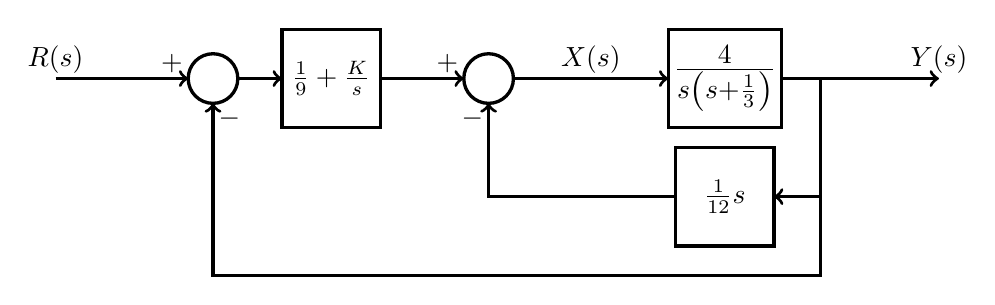
\begin{tikzpicture}[scale=1,inner sep=0pt,outer sep=0pt,very thick,
sysblock/.style={draw,rectangle,inner sep=2pt,minimum width=1.25cm,minimum height=1.25cm,very thick}]
\draw (2,0) node[draw,circle] (sum1) {$\rule{0pt}{18pt}$};
\draw (3.5,0) node[sysblock] (Kp) { $\frac{1}{9}+\frac{K}{s}$};
\draw (5.5,0) node[draw,circle] (sum2) {$\rule{0pt}{18pt}$};
\draw (8.5,0) node[sysblock] (G) {\Large $\frac{4}{s\left(s+\frac{1}{3}\right)}$};
\draw (8.5,-1.5) node[sysblock] (Kd) {$\frac{1}{12}s$};
\draw[->] (0,0) node[above=2pt] {$R(s)$} -- (sum1.180) node[above left=2pt] {$+$};
\draw[->] (sum1.0) --  (Kp);
\draw[->] (Kp) -- (sum2.180) node[above left=2pt] {$+$};
\draw[->] (sum2.0) -- node[pos=.5,above=2pt] {$X(s)$} (G.180);
\draw[->] (G.0) -- ++(2,0) node[above=2pt] {$Y(s)$};
\draw[->] (G.0) ++(0.5,0) |- (Kd.0);
\draw[->] (Kd.180) -| (sum2.-90) node[below left=2pt] {$-$};
\draw[->] (G.0) ++(0.5,0) -- ++(0,-2.5) -| (sum1.-90) node[below right=2pt] {$-$};
\end{tikzpicture}
\end{center}

\begin{enumerate}[(a)]
%\setlength{\itemsep}{3in}
%\setlength{\parskip}{0pt}
%\setlength{\parsep}{0pt}
\item If the error signal is $e(t)=r(t)-y(t)$, what is the steady state error when the reference is a unit ramp ($r(t)=tu(t)$) and $K=0.01$?
\item What is the largest value of $K$ for which there is a stable closed loop system?
\end{enumerate}

